% =====================================================================
%  Random Walks & Markov Chains: The Hidden Math of Machine Learning
%  Beamer deck  ::  compile with  pdflatex  (run twice)
%  Self-contained: all diagrams are TikZ, all charts are PGFPlots.
% =====================================================================
\documentclass[aspectratio=169,10pt]{beamer}

\usepackage[T1]{fontenc}
\usepackage{helvet}
\renewcommand{\familydefault}{\sfdefault}
\usepackage{amsmath,amssymb}
\usepackage{tikz}
\usepackage{pgfplots}
\usetikzlibrary{positioning,calc,shapes.geometric,arrows,backgrounds,fit,decorations.pathmorphing}
\pgfplotsset{compat=1.16}

% ---------------------------- palette ---------------------------------
\definecolor{cNavy}{HTML}{0F172A}
\definecolor{cNavy2}{HTML}{1E293B}
\definecolor{cTeal}{HTML}{0D9488}
\definecolor{cTealL}{HTML}{5EEAD4}
\definecolor{cPurple}{HTML}{7C3AED}
\definecolor{cPurpleD}{HTML}{312E81}
\definecolor{cPink}{HTML}{DB2777}
\definecolor{cAmber}{HTML}{F59E0B}
\definecolor{cSlate}{HTML}{64748B}
\definecolor{cLight}{HTML}{F1F5F9}
\definecolor{cInk}{HTML}{1E293B}

% ---------------------------- theme -----------------------------------
\setbeamertemplate{navigation symbols}{}
\usefonttheme{professionalfonts}
\setbeamercolor{normal text}{fg=cInk}
\setbeamercolor{itemize item}{fg=cTeal}
\setbeamercolor{itemize subitem}{fg=cPurple}
\setbeamertemplate{itemize item}{\small\textbullet}
\setbeamertemplate{itemize subitem}{\footnotesize\textendash}
\setbeamertemplate{blocks}[rounded][shadow=true]

% kicker mechanism for frame titles
\newif\ifkick \kickfalse
\newcommand{\kick}[1]{\def\thekicker{#1}\kicktrue}
\setbeamertemplate{frametitle}{%
  \vspace*{0.55em}%
  \ifkick{\color{cTeal}\scriptsize\bfseries\MakeUppercase{\thekicker}\par\vspace{1pt}}\fi%
  {\color{cInk}\large\bfseries\insertframetitle\par}%
  \vspace{0.15em}\kickfalse%
}

% generic coloured rounded block
\newenvironment{cblock}[2]{%
  \setbeamercolor{block title}{bg=#1,fg=white}%
  \setbeamercolor{block body}{bg=cLight,fg=cInk}%
  \begin{block}{#2}}{\end{block}}

% dark-navy block (for use on light slides)
\newenvironment{dblock}[2]{%
  \setbeamercolor{block title}{bg=#1,fg=white}%
  \setbeamercolor{block body}{bg=cNavy,fg=white}%
  \begin{block}{#2}}{\end{block}}

% coloured cells for the MDP mapping table
\newcommand{\boxg}[1]{\colorbox{cNavy2}{\makebox[3.0cm][l]{\color{white}\bfseries\small\,#1}}}
\newcommand{\boxr}[1]{\colorbox{cPurpleD}{\makebox[3.2cm][l]{\color{white}\bfseries\small\,#1}}}
\newcommand{\mean}[1]{{\small\color{cSlate}#1}}

% tikz styles
\tikzset{
  st/.style={circle,draw=cSlate,line width=1pt,minimum size=0.9cm,font=\bfseries\small,fill=white,inner sep=0pt},
  stwin/.style={circle,draw=cTeal,line width=1pt,minimum size=0.9cm,font=\bfseries\small,fill=cTeal,text=white,inner sep=0pt},
  struin/.style={circle,draw=cPink,line width=1pt,minimum size=0.9cm,font=\bfseries\small,fill=cPink,text=white,inner sep=0pt},
  pin/.style={->,>=stealth,line width=1.1pt,cTeal},
  qin/.style={->,>=stealth,line width=1.1pt,cPink},
}

% pgfplots clean look
\pgfplotsset{
  every axis/.append style={
    axis lines=left,
    axis line style={draw=cSlate!55,line width=0.5pt},
    tick label style={font=\tiny,color=cSlate},
    label style={font=\scriptsize,color=cInk},
    ymajorgrids=true,
    grid style={draw=cSlate!18,line width=0.4pt},
    legend style={draw=none,fill=none,font=\tiny},
    every axis plot/.append style={line width=1.1pt},
  }
}

% divider frame :  #1 num  #2 accent  #3 kicker  #4 title  #5 subtitle
\newcommand{\dividerframe}[5]{%
\begin{frame}[plain]
\begin{tikzpicture}[remember picture,overlay]
  \fill[cNavy] (current page.south west) rectangle (current page.north east);
  \fill[#2,opacity=0.16] ([xshift=1cm]current page.east) circle (3.0cm);
  \node[anchor=north west,text=#2,font=\fontsize{86}{86}\selectfont\bfseries]
     at ([shift={(0.9cm,-0.7cm)}]current page.north west) {0#1};
  \node[anchor=west,text=#2,font=\scriptsize\bfseries]
     at ([shift={(1.0cm,0.55cm)}]current page.west) {\MakeUppercase{#3}};
  \node[anchor=west,text=white,font=\LARGE\bfseries,text width=10.5cm,align=left]
     at ([shift={(1.0cm,-0.15cm)}]current page.west) {#4};
  \node[anchor=west,text=cTealL,font=\itshape\normalsize,text width=10.5cm,align=left]
     at ([shift={(1.0cm,-1.6cm)}]current page.west) {#5};
\end{tikzpicture}
\end{frame}}

% ======================================================================
\title{Random Walks \& Markov Chains}
\author{Intern PPT}
\date{}

\begin{document}

% ---------------------------------------------------------------- TITLE
\begin{frame}[plain]
\begin{tikzpicture}[remember picture,overlay]
  \fill[cNavy] (current page.south west) rectangle (current page.north east);
  % random-walk motif
  \begin{scope}[shift={([shift={(-3.4cm,0.4cm)}]current page.east)}]
    \draw[cTeal,line width=1.3pt]
       (0,0)--(0.7,-0.7)--(1.4,0)--(2.1,-0.9)--(2.8,-0.4)--(3.5,-1.3)--(4.2,-0.8);
    \foreach \x/\y/\c in {0/0/cTealL,0.7/-0.7/cPurple,1.4/0/cPink,2.1/-0.9/cAmber,2.8/-0.4/cTeal,3.5/-1.3/cTealL,4.2/-0.8/cPink}
       \fill[\c] (\x,\y) circle (2.4pt);
  \end{scope}
  \node[anchor=west,text=cTealL,font=\scriptsize\bfseries]
     at ([shift={(0.95cm,2.0cm)}]current page.west) {INTERN TECH SESSION \ \textbullet\ \ PROBABILITY $\rightarrow$ ML};
  \node[anchor=west,text=white,font=\fontsize{30}{34}\selectfont\bfseries]
     at ([shift={(0.9cm,1.15cm)}]current page.west) {Random Walks \&};
  \node[anchor=west,text=cTealL,font=\fontsize{30}{34}\selectfont\bfseries]
     at ([shift={(0.9cm,0.35cm)}]current page.west) {Markov Chains};
  \node[anchor=west,text=cLight,font=\itshape\large]
     at ([shift={(0.95cm,-0.55cm)}]current page.west) {The hidden math running your ML models};
  \node[anchor=west,text=cSlate,font=\small]
     at ([shift={(0.95cm,-1.3cm)}]current page.west)
     {From a gambler flipping a coin\ \ $\rightarrow$\ \ value iteration, PageRank \& MCMC};
  \node[anchor=west,text=cSlate,font=\footnotesize]
     at ([shift={(0.95cm,-2.55cm)}]current page.west)
     {4 problems\ \ \textbullet\ \ 1 unifying idea};
\end{tikzpicture}
\end{frame}

% ------------------------------------------------------------- WHY CARE
\begin{frame}[t]{Why should an ML team care about a gambler?}
\kick{The hook}
\small
Every system below is the \textbf{same mathematical object} in a different costume: a process that hops between states, where the next step depends only on where you are \emph{now}.
\vspace{0.6em}
\begin{columns}[t,onlytextwidth]
  \begin{column}{0.235\textwidth}
    \begin{cblock}{cPurple}{Reinforcement Learning}\scriptsize An agent choosing actions \emph{is} a gambler choosing bets. Value iteration solves it.\end{cblock}
  \end{column}
  \begin{column}{0.235\textwidth}
    \begin{cblock}{cTeal}{Google PageRank}\scriptsize A surfer clicking links at random; page rank $=$ the stationary distribution.\end{cblock}
  \end{column}
  \begin{column}{0.235\textwidth}
    \begin{cblock}{cPink}{Bayesian / MCMC}\scriptsize Sampling an impossible posterior $=$ a Markov chain that lands where you want.\end{cblock}
  \end{column}
  \begin{column}{0.235\textwidth}
    \begin{cblock}{cAmber}{Quant Finance}\scriptsize Stock prices, ruin probability, risk of bankruptcy.\end{cblock}
  \end{column}
\end{columns}
\vspace{0.7em}
\footnotesize\textit{\textbf{\textcolor{cTeal}{Big idea:}} learn it once on a toy gambling problem, and a huge slice of modern ML comes for free.}
\end{frame}

% -------------------------------------------------------------- ROADMAP
\begin{frame}[t]{Where we're going}
\kick{Roadmap}
\small Four stations. Each one is a question from the assignment, opened up into a real-world problem.
\vspace{0.7em}
\begin{columns}[t,onlytextwidth]
  \begin{column}{0.235\textwidth}
    \begin{cblock}{cTeal}{1\ \ The Random Walk}\scriptsize A gambler, a coin, two walls. The atom of everything.\end{cblock}
  \end{column}
  \begin{column}{0.235\textwidth}
    \begin{cblock}{cPurple}{2\ \ Walk $\to$ Decision}\scriptsize Add choices \& rewards: the gambler becomes an RL agent.\end{cblock}
  \end{column}
  \begin{column}{0.235\textwidth}
    \begin{cblock}{cPink}{3\ \ Walls \& Constraints}\scriptsize Bounded walks, reflecting barriers, modular arithmetic.\end{cblock}
  \end{column}
  \begin{column}{0.235\textwidth}
    \begin{cblock}{cAmber}{4\ \ Stationary World}\scriptsize Where do you end up long-run? PageRank \& MCMC.\end{cblock}
  \end{column}
\end{columns}
\vspace{0.8em}
\centering\footnotesize\textit{\textcolor{cSlate}{Learn the atom once --- recognise it everywhere.}}
\end{frame}

% ============================================================ DIVIDER 1
\dividerframe{1}{cTeal}{Station 1}{The Random Walk}{One coin, one number line, two absorbing walls --- the simplest stochastic process there is.}

% ----------------------------------------------------- S1: state chain
\begin{frame}[t]{A gambler on a number line}
\kick{Station 1 \ \textbullet\ \ the object}
\small Start with $k$ dollars. Each round, a biased coin: \textcolor{cTeal}{\textbf{$+1$ with prob.\ $p$}}, \textcolor{cPink}{\textbf{$-1$ with prob.\ $q=1-p$}}. Stop at \textcolor{cPink}{\textbf{$0$ (ruin)}} or \textcolor{cTeal}{\textbf{$N$ (win)}}.
\vspace{0.3em}
\begin{center}
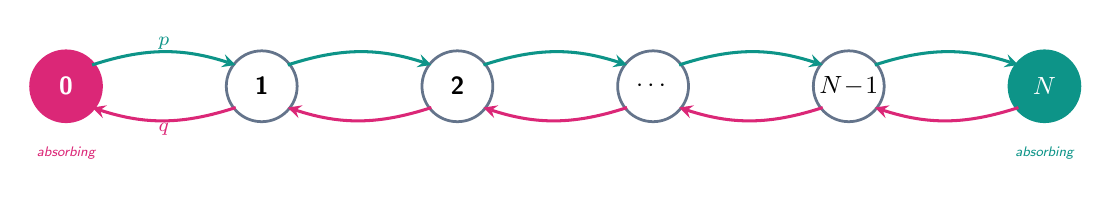
\begin{tikzpicture}[node distance=1.55cm]
  \node[struin] (s0) {0};
  \node[st,right=of s0] (s1) {1};
  \node[st,right=of s1] (s2) {2};
  \node[st,right=of s2] (sd) {$\cdots$};
  \node[st,right=of sd] (sn1) {$N\!-\!1$};
  \node[stwin,right=of sn1] (sn) {$N$};
  \foreach \a/\b in {s0/s1,s1/s2,s2/sd,sd/sn1,sn1/sn}
     \draw[pin] ($(\a.north east)+(0,-0.06)$) to[bend left=18] ($(\b.north west)+(0,-0.06)$);
  \foreach \a/\b in {s1/s0,s2/s1,sd/s2,sn1/sd,sn/sn1}
     \draw[qin] ($(\a.south west)+(0,0.06)$) to[bend left=18] ($(\b.south east)+(0,0.06)$);
  \node[cTeal,font=\scriptsize\bfseries] at ($(s0)!0.5!(s1)+(0,0.55)$) {$p$};
  \node[cPink,font=\scriptsize\bfseries] at ($(s0)!0.5!(s1)+(0,-0.55)$) {$q$};
  \node[cPink,font=\tiny\itshape] at ($(s0)+(0,-0.85)$) {absorbing};
  \node[cTeal,font=\tiny\itshape] at ($(sn)+(0,-0.85)$) {absorbing};
\end{tikzpicture}
\end{center}
\vspace{0.1em}
\begin{columns}[t,onlytextwidth]
  \begin{column}{0.46\textwidth}
    \begin{cblock}{cPurple}{The Markov property}\scriptsize The next state depends \emph{only} on the current wealth --- not on the path taken. Memoryless. This single assumption makes everything solvable.\end{cblock}
  \end{column}
  \begin{column}{0.5\textwidth}
    \begin{dblock}{cTeal}{One recurrence to rule them all}
      \centering\color{white}$T(k)=p\,T(k{+}1)+q\,T(k{-}1)$
      \par\vspace{2pt}\scriptsize\color{cTealL}\itshape with $T(0)=0,\ T(N)=1$
    \end{dblock}
  \end{column}
\end{columns}
\end{frame}

% ----------------------------------------------------- S1: win prob
\begin{frame}[t]{Will she win? A closed-form probability}
\kick{Station 1 \ \textbullet\ \ the answer}
\begin{columns}[t,onlytextwidth]
  \begin{column}{0.45\textwidth}
    \begin{dblock}{cTeal}{Win probability $T(k)$}
      \color{white}\centering
      unfair $(p\neq q)$:\\[1pt]
      $\displaystyle T(k)=\frac{1-(q/p)^{k}}{1-(q/p)^{N}}$\\[3pt]
      fair $(p=q=\tfrac12)$:\ \ $\displaystyle T(k)=\frac{k}{N}$
    \end{dblock}
    \vspace{0.2em}
    {\scriptsize\textbf{\textcolor{cPink}{Casino edge.}} At $p{=}0.45$ (a mere $5\%$ house edge), from the halfway point your win chance \textbf{collapses toward zero} as $N$ grows.}
  \end{column}
  \begin{column}{0.52\textwidth}
    \centering
    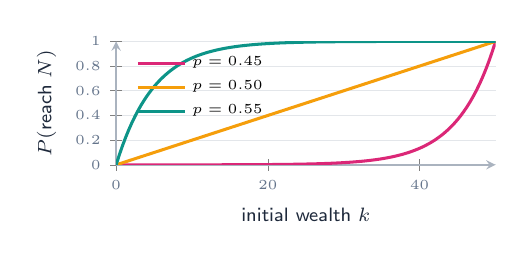
\begin{tikzpicture}
    \begin{axis}[width=6.4cm,height=3.15cm,xlabel={initial wealth $k$},
        ylabel={$P(\text{reach }N)$},xmin=0,xmax=50,ymin=0,ymax=1,
        legend pos=north west,legend cell align=left]
      \addplot[cPink,domain=0:50,samples=120]{(1-(0.55/0.45)^x)/(1-(0.55/0.45)^50)};
      \addlegendentry{$p=0.45$}
      \addplot[cAmber,domain=0:50,samples=2]{x/50};
      \addlegendentry{$p=0.50$}
      \addplot[cTeal,domain=0:50,samples=120]{(1-(0.45/0.55)^x)/(1-(0.45/0.55)^50)};
      \addlegendentry{$p=0.55$}
    \end{axis}
    \end{tikzpicture}\\[2pt]
    {\scriptsize\textbf{\textcolor{cTeal}{ML echo.}} A barely-better-than-chance classifier, chained over many decisions, can still fail catastrophically.}
  \end{column}
\end{columns}
\end{frame}

% ----------------------------------------------------- S1: trajectories
\begin{frame}[t]{Six gamblers, three coins}
\kick{Station 1 \ \textbullet\ \ see it move}
\small Each line is one simulated life: start at wealth $25$, walls at $0$ and $50$. Same rules, wildly different fates.
\vspace{0.2em}
\begin{columns}[t,onlytextwidth]
  \begin{column}{0.32\textwidth}
    \centering
    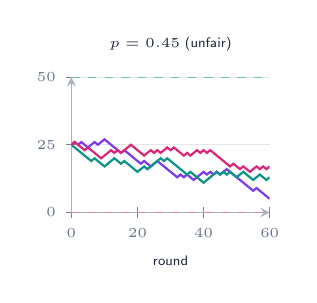
\begin{tikzpicture}
    \begin{axis}[width=4.1cm,height=3.3cm,xmin=0,xmax=60,ymin=0,ymax=50,title={\tiny\color{cInk}$p=0.45$ (unfair)},xlabel={\tiny round},ytick={0,25,50}]
      \draw[dashed,cTeal!60] (axis cs:0,50)--(axis cs:60,50);
      \draw[dashed,cPink!60] (axis cs:0,0)--(axis cs:60,0);
      \addplot[cPurple,line width=0.8pt] coordinates {(0,25) (1,26) (2,25) (3,26) (4,25) (5,24) (6,25) (7,26) (8,25) (9,26) (10,27) (11,26) (12,25) (13,24) (14,23) (15,22) (16,23) (17,22) (18,21) (19,20) (20,19) (21,18) (22,19) (23,18) (24,17) (25,18) (26,19) (27,18) (28,17) (29,16) (30,15) (31,14) (32,13) (33,14) (34,13) (35,14) (36,13) (37,12) (38,13) (39,14) (40,15) (41,14) (42,15) (43,14) (44,15) (45,14) (46,15) (47,16) (48,15) (49,14) (50,13) (51,12) (52,11) (53,10) (54,9) (55,8) (56,9) (57,8) (58,7) (59,6) (60,5)};
      \addplot[cTeal,line width=0.8pt] coordinates {(0,25) (1,24) (2,23) (3,22) (4,21) (5,20) (6,19) (7,20) (8,19) (9,18) (10,17) (11,18) (12,19) (13,20) (14,19) (15,18) (16,19) (17,18) (18,17) (19,16) (20,15) (21,16) (22,17) (23,16) (24,17) (25,18) (26,19) (27,20) (28,19) (29,20) (30,19) (31,18) (32,17) (33,16) (34,15) (35,14) (36,15) (37,14) (38,13) (39,12) (40,11) (41,12) (42,13) (43,14) (44,15) (45,14) (46,15) (47,14) (48,15) (49,14) (50,13) (51,14) (52,15) (53,14) (54,13) (55,12) (56,13) (57,14) (58,13) (59,12) (60,13)};
      \addplot[cPink,line width=0.8pt] coordinates {(0,25) (1,26) (2,25) (3,24) (4,23) (5,24) (6,23) (7,22) (8,21) (9,20) (10,21) (11,22) (12,23) (13,22) (14,23) (15,22) (16,23) (17,24) (18,25) (19,24) (20,23) (21,22) (22,21) (23,22) (24,23) (25,22) (26,23) (27,22) (28,23) (29,24) (30,23) (31,24) (32,23) (33,22) (34,21) (35,22) (36,21) (37,22) (38,23) (39,22) (40,23) (41,22) (42,23) (43,22) (44,21) (45,20) (46,19) (47,18) (48,17) (49,18) (50,17) (51,16) (52,17) (53,16) (54,15) (55,16) (56,17) (57,16) (58,17) (59,16) (60,17)};
    \end{axis}
    \end{tikzpicture}\\[1pt]
    {\tiny\color{cSlate}\itshape slight disadvantage drags everyone to ruin}
  \end{column}
  \begin{column}{0.32\textwidth}
    \centering
    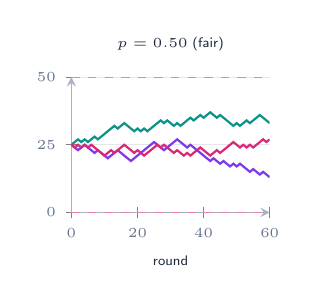
\begin{tikzpicture}
    \begin{axis}[width=4.1cm,height=3.3cm,xmin=0,xmax=60,ymin=0,ymax=50,title={\tiny\color{cInk}$p=0.50$ (fair)},xlabel={\tiny round},ytick={0,25,50}]
      \draw[dashed,cTeal!60] (axis cs:0,50)--(axis cs:60,50);
      \draw[dashed,cPink!60] (axis cs:0,0)--(axis cs:60,0);
      \addplot[cPurple,line width=0.8pt] coordinates {(0,25) (1,24) (2,23) (3,24) (4,25) (5,24) (6,23) (7,22) (8,23) (9,22) (10,21) (11,20) (12,21) (13,22) (14,23) (15,22) (16,21) (17,20) (18,19) (19,20) (20,21) (21,22) (22,23) (23,24) (24,25) (25,26) (26,25) (27,24) (28,23) (29,24) (30,25) (31,26) (32,27) (33,26) (34,25) (35,24) (36,25) (37,24) (38,23) (39,22) (40,21) (41,20) (42,19) (43,20) (44,19) (45,18) (46,19) (47,18) (48,17) (49,18) (50,17) (51,18) (52,17) (53,16) (54,15) (55,16) (56,15) (57,14) (58,15) (59,14) (60,13)};
      \addplot[cTeal,line width=0.8pt] coordinates {(0,25) (1,26) (2,27) (3,26) (4,27) (5,26) (6,27) (7,28) (8,27) (9,28) (10,29) (11,30) (12,31) (13,32) (14,31) (15,32) (16,33) (17,32) (18,31) (19,30) (20,31) (21,30) (22,31) (23,30) (24,31) (25,32) (26,33) (27,34) (28,33) (29,34) (30,33) (31,32) (32,33) (33,32) (34,33) (35,34) (36,35) (37,34) (38,35) (39,36) (40,35) (41,36) (42,37) (43,36) (44,35) (45,36) (46,35) (47,34) (48,33) (49,32) (50,33) (51,32) (52,33) (53,34) (54,33) (55,34) (56,35) (57,36) (58,35) (59,34) (60,33)};
      \addplot[cPink,line width=0.8pt] coordinates {(0,25) (1,24) (2,25) (3,24) (4,25) (5,24) (6,25) (7,24) (8,23) (9,22) (10,21) (11,22) (12,23) (13,22) (14,23) (15,24) (16,25) (17,24) (18,23) (19,22) (20,23) (21,22) (22,21) (23,22) (24,23) (25,24) (26,25) (27,24) (28,25) (29,24) (30,23) (31,22) (32,23) (33,22) (34,21) (35,22) (36,21) (37,22) (38,23) (39,24) (40,23) (41,22) (42,21) (43,22) (44,23) (45,22) (46,23) (47,24) (48,25) (49,26) (50,25) (51,24) (52,25) (53,24) (54,25) (55,24) (56,25) (57,26) (58,27) (59,26) (60,27)};
    \end{axis}
    \end{tikzpicture}\\[1pt]
    {\tiny\color{cSlate}\itshape a coin-flip of destinies}
  \end{column}
  \begin{column}{0.32\textwidth}
    \centering
    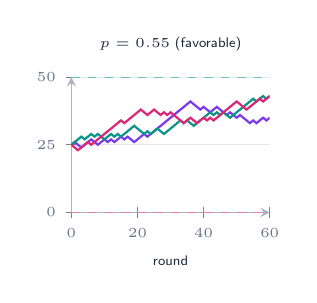
\begin{tikzpicture}
    \begin{axis}[width=4.1cm,height=3.3cm,xmin=0,xmax=60,ymin=0,ymax=50,title={\tiny\color{cInk}$p=0.55$ (favorable)},xlabel={\tiny round},ytick={0,25,50}]
      \draw[dashed,cTeal!60] (axis cs:0,50)--(axis cs:60,50);
      \draw[dashed,cPink!60] (axis cs:0,0)--(axis cs:60,0);
      \addplot[cPurple,line width=0.8pt] coordinates {(0,25) (1,26) (2,25) (3,24) (4,25) (5,26) (6,27) (7,26) (8,25) (9,26) (10,27) (11,26) (12,27) (13,26) (14,27) (15,28) (16,27) (17,28) (18,27) (19,26) (20,27) (21,28) (22,29) (23,28) (24,29) (25,30) (26,31) (27,32) (28,33) (29,34) (30,35) (31,36) (32,37) (33,38) (34,39) (35,40) (36,41) (37,40) (38,39) (39,38) (40,39) (41,38) (42,37) (43,38) (44,39) (45,38) (46,37) (47,36) (48,37) (49,36) (50,35) (51,36) (52,35) (53,34) (54,33) (55,34) (56,33) (57,34) (58,35) (59,34) (60,35)};
      \addplot[cTeal,line width=0.8pt] coordinates {(0,25) (1,26) (2,27) (3,28) (4,27) (5,28) (6,29) (7,28) (8,29) (9,28) (10,27) (11,28) (12,29) (13,28) (14,29) (15,28) (16,29) (17,30) (18,31) (19,32) (20,31) (21,30) (22,29) (23,30) (24,29) (25,30) (26,31) (27,30) (28,29) (29,30) (30,31) (31,32) (32,33) (33,34) (34,33) (35,34) (36,33) (37,32) (38,33) (39,34) (40,35) (41,36) (42,37) (43,36) (44,37) (45,36) (46,37) (47,36) (48,35) (49,36) (50,37) (51,38) (52,39) (53,40) (54,41) (55,42) (56,41) (57,42) (58,43) (59,42) (60,43)};
      \addplot[cPink,line width=0.8pt] coordinates {(0,25) (1,24) (2,23) (3,24) (4,25) (5,26) (6,25) (7,26) (8,27) (9,28) (10,29) (11,30) (12,31) (13,32) (14,33) (15,34) (16,33) (17,34) (18,35) (19,36) (20,37) (21,38) (22,37) (23,36) (24,37) (25,38) (26,37) (27,36) (28,37) (29,36) (30,37) (31,36) (32,35) (33,34) (34,33) (35,34) (36,35) (37,34) (38,33) (39,34) (40,35) (41,34) (42,35) (43,34) (44,35) (45,36) (46,37) (47,38) (48,39) (49,40) (50,41) (51,40) (52,39) (53,38) (54,39) (55,40) (56,41) (57,42) (58,41) (59,42) (60,43)};
    \end{axis}
    \end{tikzpicture}\\[1pt]
    {\tiny\color{cSlate}\itshape a slight edge, most paths climb}
  \end{column}
\end{columns}
\end{frame}

% ============================================================ DIVIDER 2
\dividerframe{2}{cPurple}{Station 2}{From Walk to Decision}{What if the gambler could \emph{choose} her bets? Welcome to Reinforcement Learning.}

% ----------------------------------------------------- S2: the leap
\begin{frame}[t]{Add a choice, and probability becomes intelligence}
\kick{Station 2 \ \textbullet\ \ the leap}
\begin{columns}[t,onlytextwidth]
  \begin{column}{0.48\textwidth}
    \begin{cblock}{cTeal}{Passive walk\ \ (Assignment Q1--Q2)}\scriptsize
      The bet is \textbf{fixed} (\$1, or all-in in Q2). The gambler has no agency.\\[3pt]
      We ask: \textit{``given the rules, what is my probability of winning?''}\\[3pt]
      \textbf{\textcolor{cTeal}{$\Rightarrow$ Prediction}} (policy evaluation).
    \end{cblock}
  \end{column}
  \begin{column}{0.48\textwidth}
    \begin{cblock}{cPurple}{Active agent\ \ (the RL upgrade)}\scriptsize
      At each state the agent \textbf{chooses} how much to bet --- a decision at every step.\\[3pt]
      We ask: \textit{``which strategy \emph{maximises} my chance of winning?''}\\[3pt]
      \textbf{\textcolor{cPurple}{$\Rightarrow$ Control}} --- finding the optimal policy $\pi^{*}$.
    \end{cblock}
  \end{column}
\end{columns}
\vspace{0.6em}
\centering\footnotesize\textit{This exact problem --- ``The Gambler's Problem'' --- is \textbf{\textcolor{cPurple}{Example 4.3 in Sutton \& Barto}}, the standard RL textbook.}
\end{frame}

% ----------------------------------------------------- S2: MDP table
\begin{frame}[t]{Your gambler \emph{is} a Markov Decision Process}
\kick{Station 2 \ \textbullet\ \ the rosetta stone}
\vspace{0.3em}
\setlength{\fboxsep}{4pt}
\renewcommand{\arraystretch}{1.55}
\begin{tabular}{@{}l l l@{}}
\textcolor{cTeal}{\scriptsize\bfseries GAMBLER} & \textcolor{cPurple}{\scriptsize\bfseries RL / MDP} & \textcolor{cAmber}{\scriptsize\bfseries MEANING}\\
\boxg{Wealth $k$}        & \boxr{State $s$}              & \mean{where the agent currently is}\\
\boxg{Bet size}          & \boxr{Action $a$}             & \mean{what the agent decides to do}\\
\boxg{Coin $p,q$}        & \boxr{Transition $P(s'|s,a)$} & \mean{the environment's dynamics}\\
\boxg{Reaching $N$}      & \boxr{Reward $r=+1$}          & \mean{the goal signal}\\
\boxg{Win prob.\ $T(k)$} & \boxr{Value $V(s)$}           & \mean{``how good is this state?''}\\
\boxg{Best bet rule}     & \boxr{Policy $\pi^{*}(s)$}    & \mean{the learned strategy}\\
\end{tabular}
\end{frame}

% ----------------------------------------------------- S2: Bellman + VI
\begin{frame}[t]{Same recurrence, one tiny twist: a max}
\kick{Station 2 \ \textbullet\ \ how machines solve it}
\begin{columns}[t,onlytextwidth]
  \begin{column}{0.46\textwidth}
    \begin{dblock}{cTeal}{From assignment $\to$ Bellman}\scriptsize\color{white}
      Your recurrence:\\[1pt] $\displaystyle T(k)=p\,T(k{+}1)+q\,T(k{-}1)$\\[5pt]
      \color{cTealL}Bellman optimality:\\[1pt] \color{white}$\displaystyle V(s)=\max_{a}\big[\,p\,V(s{+}a)+q\,V(s{-}a)\,\big]$
    \end{dblock}
    \begin{cblock}{cPurple}{Value iteration}\scriptsize
      \begin{enumerate}\setlength\itemsep{1pt}
        \item Guess $V(s)$ for every state.
        \item Sweep: update each state with the Bellman max.
        \item Repeat until $V$ converges.
        \item Read off the maximising bet $\to \pi^{*}$.
      \end{enumerate}
    \end{cblock}
  \end{column}
  \begin{column}{0.5\textwidth}
    \centering
    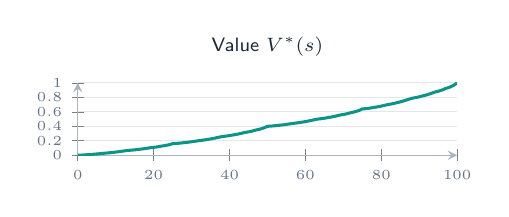
\begin{tikzpicture}
    \begin{axis}[width=6.4cm,height=2.5cm,title={\scriptsize\color{cInk}Value $V^{*}(s)$},
        xmin=0,xmax=100,ymin=0,ymax=1,xlabel={},ylabel={}]
      \addplot[cTeal] coordinates {(0,0.00000) (1,0.00207) (2,0.00516) (3,0.00923) (4,0.01291) (5,0.01739) (6,0.02306) (7,0.02781) (8,0.03228) (9,0.03769) (10,0.04346) (11,0.05035) (12,0.05766) (13,0.06524) (14,0.06954) (15,0.07443) (16,0.08069) (17,0.08661) (18,0.09421) (19,0.10314) (20,0.10866) (21,0.11597) (22,0.12589) (23,0.13358) (24,0.14415) (25,0.16000) (26,0.16310) (27,0.16775) (28,0.17384) (29,0.17937) (30,0.18608) (31,0.19460) (32,0.20172) (33,0.20841) (34,0.21653) (35,0.22520) (36,0.23553) (37,0.24649) (38,0.25786) (39,0.26430) (40,0.27165) (41,0.28103) (42,0.28992) (43,0.30132) (44,0.31472) (45,0.32299) (46,0.33395) (47,0.34883) (48,0.36037) (49,0.37622) (50,0.40000) (51,0.40310) (52,0.40775) (53,0.41384) (54,0.41937) (55,0.42608) (56,0.43460) (57,0.44172) (58,0.44841) (59,0.45653) (60,0.46520) (61,0.47553) (62,0.48649) (63,0.49786) (64,0.50430) (65,0.51165) (66,0.52103) (67,0.52992) (68,0.54132) (69,0.55472) (70,0.56299) (71,0.57395) (72,0.58883) (73,0.60037) (74,0.61622) (75,0.64000) (76,0.64465) (77,0.65162) (78,0.66076) (79,0.66905) (80,0.67912) (81,0.69189) (82,0.70258) (83,0.71262) (84,0.72479) (85,0.73779) (86,0.75330) (87,0.76973) (88,0.78679) (89,0.79645) (90,0.80747) (91,0.82155) (92,0.83487) (93,0.85198) (94,0.87207) (95,0.88448) (96,0.90092) (97,0.92324) (98,0.94055) (99,0.96433) (100,1.00000)};
    \end{axis}
    \end{tikzpicture}\\[2pt]
    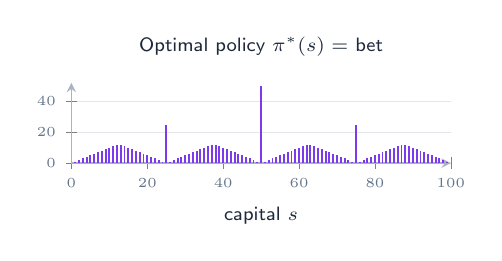
\begin{tikzpicture}
    \begin{axis}[width=6.4cm,height=2.6cm,title={\scriptsize\color{cInk}Optimal policy $\pi^{*}(s)=$ bet},
        xmin=0,xmax=100,ymin=0,ymax=52,xlabel={\scriptsize capital $s$}]
      \addplot[ycomb,cPurple,line width=0.7pt] coordinates {(1,1) (2,2) (3,3) (4,4) (5,5) (6,6) (7,7) (8,8) (9,9) (10,10) (11,11) (12,12) (13,12) (14,11) (15,10) (16,9) (17,8) (18,7) (19,6) (20,5) (21,4) (22,3) (23,2) (24,1) (25,25) (26,1) (27,2) (28,3) (29,4) (30,5) (31,6) (32,7) (33,8) (34,9) (35,10) (36,11) (37,12) (38,12) (39,11) (40,10) (41,9) (42,8) (43,7) (44,6) (45,5) (46,4) (47,3) (48,2) (49,1) (50,50) (51,1) (52,2) (53,3) (54,4) (55,5) (56,6) (57,7) (58,8) (59,9) (60,10) (61,11) (62,12) (63,12) (64,11) (65,10) (66,9) (67,8) (68,7) (69,6) (70,5) (71,4) (72,3) (73,2) (74,1) (75,25) (76,1) (77,2) (78,3) (79,4) (80,5) (81,6) (82,7) (83,8) (84,9) (85,10) (86,11) (87,12) (88,12) (89,11) (90,10) (91,9) (92,8) (93,7) (94,6) (95,5) (96,4) (97,3) (98,2) (99,1)};
    \end{axis}
    \end{tikzpicture}\\[1pt]
    {\scriptsize\color{cSlate}\itshape Bold, all-or-nothing betting at $50,25,75,\dots$ --- the value function is famously \textbf{fractal} (arXiv:2001.00102).}
  \end{column}
\end{columns}
\end{frame}

% ----------------------------------------------------- S2: binary trick
\begin{frame}[t]{Bold play \& the binary-expansion shortcut}
\kick{Station 2 \ \textbullet\ \ the slick trick}
\small Q2's aggressive gambler bets everything below $N/2$. Writing $k/N$ in binary turns the whole recursion into bit-shifting.
\vspace{0.3em}
\begin{columns}[t,onlytextwidth]
  \begin{column}{0.49\textwidth}
    \begin{dblock}{cTeal}{The rule, in bits of $k/N=.b_1b_2b_3\dots$}\footnotesize\color{white}
      \textcolor{cTealL}{\textbf{bit $=0$}}\ \ $\to\ P(x)=p\cdot P(2x)$\\[3pt]
      \hspace*{2.6em}{\scriptsize(shift left, $\times p$)}\\[6pt]
      \textcolor{cPink}{\textbf{bit $=1$}}\ \ $\to\ P(x)=q\cdot P(2x{-}N)+p$\\[3pt]
      \hspace*{2.6em}{\scriptsize(shift, drop a bit, $\times q$, $+p$)}
    \end{dblock}
  \end{column}
  \begin{column}{0.49\textwidth}
    \begin{cblock}{cAmber}{Why an ML team should grin}\scriptsize
      \textbf{Change of representation.} The right basis (here: binary) collapses complexity --- the instinct behind feature engineering \& embeddings.\\[4pt]
      \textbf{Bold vs.\ timid play.} Under bad odds, high-variance strategies win --- counterintuitive but provable.\\[4pt]
      \textbf{Exact, not approximate.} Structure gives a closed form; no neural net needed.
    \end{cblock}
  \end{column}
\end{columns}
\end{frame}

% ============================================================ DIVIDER 3
\dividerframe{3}{cPink}{Station 3}{Walls, Curses \& Constraints}{Reflecting barriers, capped wealth, and answers mod $10^9{+}7$ --- when the real world adds rules.}

% ----------------------------------------------------- S3: reflecting
\begin{frame}[t]{A ceiling on luck: reflecting boundaries}
\kick{Station 3 \ \textbullet\ \ the cursed gambler}
\small Q3's gambler is cursed: once she touches wealth $m$, she can never pass $m{+}W$ --- at the top she is bounced back. How many rounds until she quits at $t$?
\vspace{0.2em}
\begin{center}
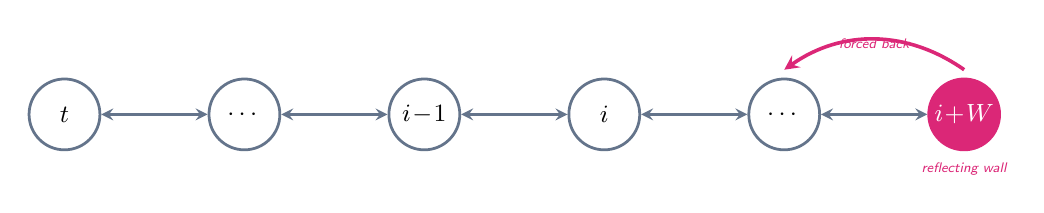
\begin{tikzpicture}[node distance=1.35cm]
  \node[st] (t) {$t$};
  \node[st,right=of t] (a) {$\cdots$};
  \node[st,right=of a] (b) {$i\!-\!1$};
  \node[st,right=of b] (c) {$i$};
  \node[st,right=of c] (d) {$\cdots$};
  \node[struin,right=of d] (w) {$i\!+\!W$};
  \foreach \a/\b in {t/a,a/b,b/c,c/d,d/w} \draw[<->,>=stealth,line width=0.9pt,cSlate] (\a)--(\b);
  \draw[->,>=stealth,line width=1.3pt,cPink] ($(w.north)+(0,0.1)$) to[bend right=35] ($(d.north)+(0,0.1)$);
  \node[cPink,font=\tiny\itshape] at ($(d)!0.5!(w)+(0,0.9)$) {forced back};
  \node[cPink,font=\tiny\itshape] at ($(w)+(0,-0.7)$) {reflecting wall};
\end{tikzpicture}
\end{center}
\begin{columns}[t,onlytextwidth]
  \begin{column}{0.48\textwidth}
    \begin{dblock}{cTeal}{The decomposition trick}\scriptsize\color{white}
      $E[\text{time }t\to k]=\sum E[\text{drop one level}]$ by linearity. Each drop sees the same local window of size $W$, so it is a \textbf{constant} $X$.\\[3pt]
      $\Rightarrow\ E(k)=X\cdot(k-t)$.
    \end{dblock}
  \end{column}
  \begin{column}{0.48\textwidth}
    \begin{cblock}{cPink}{Real world: bounded resources}\scriptsize
      Reflecting walls model capped buffers, rate limits, inventory ceilings, and \textbf{$\varepsilon$-greedy exploration} bouncing off an action space. ``Expected time to absorb'' $=$ expected episodes to converge.
    \end{cblock}
  \end{column}
\end{columns}
\end{frame}

% ----------------------------------------------------- S3: mod arithmetic
\begin{frame}[t]{Why ``mod $10^9{+}7$''? The detail ML lives by}
\kick{Station 3 \ \textbullet\ \ numerical stability}
\small Q3 wants the answer as $a\cdot b^{-1}\bmod(10^9{+}7)$. Strange for a probability --- until you see what it teaches.
\vspace{0.5em}
\begin{columns}[t,onlytextwidth]
  \begin{column}{0.31\textwidth}
    \begin{cblock}{cPink}{Exact arithmetic}\scriptsize Probabilities are fractions $a/b$. Floating point corrupts them after thousands of products; modular inverses stay exact.\end{cblock}
  \end{column}
  \begin{column}{0.31\textwidth}
    \begin{cblock}{cTeal}{The ML parallel}\scriptsize This \emph{is} numerical stability --- the reason for log-probabilities, the log-sum-exp trick, and fp32 accumulation. Tiny errors compound, just like the edge.\end{cblock}
  \end{column}
  \begin{column}{0.31\textwidth}
    \begin{cblock}{cAmber}{The discipline}\scriptsize Represent the same number differently (a fraction as a modular integer) to keep computation tractable. Pure engineering judgment.\end{cblock}
  \end{column}
\end{columns}
\vspace{0.7em}
\centering\footnotesize\textit{\textcolor{cTeal}{The assignment quietly trains the instinct that keeps real ML pipelines from silently producing garbage.}}
\end{frame}

% ============================================================ DIVIDER 4
\dividerframe{4}{cAmber}{Station 4}{The Stationary World}{Forget where you start --- where do you spend your time long-run? This idea powers PageRank \& MCMC.}

% ----------------------------------------------------- S4: stationary
\begin{frame}[t]{Stock prices \& the stationary distribution}
\kick{Station 4 \ \textbullet\ \ the long run}
\small Q4 models a price as a birth--death chain (up $p_k$, down $q_k$, stay $r_k$). Run it forever: the time spent at each price settles into a fixed $\pi$.
\vspace{0.1em}
\begin{columns}[c,onlytextwidth]
  \begin{column}{0.5\textwidth}
    \centering
    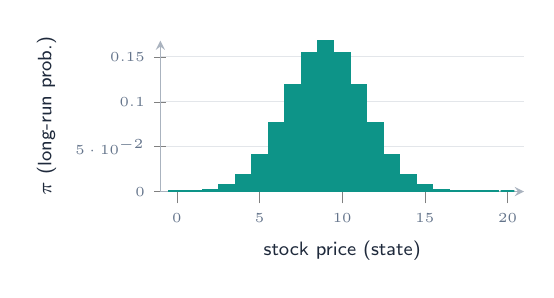
\begin{tikzpicture}
    \begin{axis}[width=6.2cm,height=3.5cm,xlabel={\scriptsize stock price (state)},
        ylabel={\scriptsize $\pi$ (long-run prob.)},xmin=-1,xmax=21,ymin=0,
        ybar,bar width=5pt]
      \addplot[fill=cTeal,draw=cTeal] coordinates {(0,0.00006) (1,0.00037) (2,0.00174) (3,0.00628) (4,0.01779) (5,0.04066) (6,0.07624) (7,0.11859) (8,0.15417) (9,0.16819) (10,0.15417) (11,0.11859) (12,0.07624) (13,0.04066) (14,0.01779) (15,0.00628) (16,0.00174) (17,0.00037) (18,0.00006) (19,0.00001) (20,0.00000)};
    \end{axis}
    \end{tikzpicture}
  \end{column}
  \begin{column}{0.46\textwidth}
    \begin{dblock}{cTeal}{The defining equation}\centering\color{white}\large $\pi=\pi P$\par
      \scriptsize\color{cTealL}\itshape left eigenvector of $P$, eigenvalue $1$\end{dblock}
    \vspace{-0.2em}
    \begin{cblock}{cAmber}{Detailed-balance recursion}\scriptsize
      $\displaystyle \pi_i=\pi_{i-1}\cdot\frac{p_{i-1}}{q_i}$,\ \ then normalise.\\[2pt]
      Read off $E[\text{price}]=\sum_i i\,\pi_i$.
    \end{cblock}
  \end{column}
\end{columns}
\end{frame}

% ----------------------------------------------------- S4: mixing
\begin{frame}[t]{Convergence: the chain forgets where it started}
\kick{Station 4 \ \textbullet\ \ mixing}
\small Start dead-certain at state $2$. Watch it spread and settle; after enough steps it forgets the start entirely. That ``forgetting'' is the engine behind sampling.
\vspace{0.2em}
\begin{columns}[t,onlytextwidth]
  \begin{column}{0.52\textwidth}
    \centering
    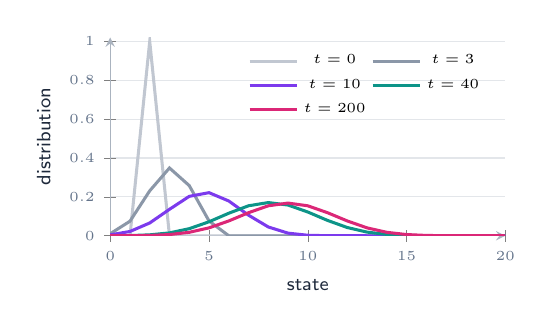
\begin{tikzpicture}
    \begin{axis}[width=6.6cm,height=4.1cm,xlabel={\scriptsize state},ylabel={\scriptsize distribution},
        xmin=0,xmax=20,ymin=0,ymax=1.02,legend pos=north east,legend columns=2]
      \addplot[cSlate!40] coordinates {(0,0.00000) (1,0.00000) (2,1.00000) (3,0.00000) (4,0.00000) (5,0.00000) (6,0.00000) (7,0.00000) (8,0.00000) (9,0.00000) (10,0.00000) (11,0.00000) (12,0.00000) (13,0.00000) (14,0.00000) (15,0.00000) (16,0.00000) (17,0.00000) (18,0.00000) (19,0.00000) (20,0.00000)};   \addlegendentry{$t=0$}
      \addplot[cSlate!75] coordinates {(0,0.01050) (1,0.07488) (2,0.23119) (3,0.34875) (4,0.25819) (5,0.07650) (6,0.00000) (7,0.00000) (8,0.00000) (9,0.00000) (10,0.00000) (11,0.00000) (12,0.00000) (13,0.00000) (14,0.00000) (15,0.00000) (16,0.00000) (17,0.00000) (18,0.00000) (19,0.00000) (20,0.00000)};   \addlegendentry{$t=3$}
      \addplot[cPurple]   coordinates {(0,0.00474) (1,0.02211) (2,0.06581) (3,0.13607) (4,0.20276) (5,0.22174) (6,0.17895) (7,0.10601) (8,0.04531) (9,0.01351) (10,0.00265) (11,0.00030) (12,0.00002) (13,0.00000) (14,0.00000) (15,0.00000) (16,0.00000) (17,0.00000) (18,0.00000) (19,0.00000) (20,0.00000)};  \addlegendentry{$t=10$}
      \addplot[cTeal]     coordinates {(0,0.00019) (1,0.00114) (2,0.00474) (3,0.01486) (4,0.03647) (5,0.07193) (6,0.11589) (7,0.15426) (8,0.17084) (9,0.15804) (10,0.12226) (11,0.07896) (12,0.04239) (13,0.01877) (14,0.00678) (15,0.00196) (16,0.00044) (17,0.00008) (18,0.00001) (19,0.00000) (20,0.00000)};  \addlegendentry{$t=40$}
      \addplot[cPink]     coordinates {(0,0.00006) (1,0.00037) (2,0.00174) (3,0.00628) (4,0.01779) (5,0.04067) (6,0.07625) (7,0.11861) (8,0.15418) (9,0.16819) (10,0.15417) (11,0.11858) (12,0.07623) (13,0.04065) (14,0.01779) (15,0.00628) (16,0.00174) (17,0.00037) (18,0.00006) (19,0.00001) (20,0.00000)}; \addlegendentry{$t=200$}
    \end{axis}
    \end{tikzpicture}
  \end{column}
  \begin{column}{0.44\textwidth}
    \begin{cblock}{cAmber}{Three conditions for a unique $\pi$}\scriptsize
      \begin{itemize}\setlength\itemsep{2pt}
        \item[\textcolor{cAmber}{\textbullet}] \textbf{Irreducible} --- reach any state from any other
        \item[\textcolor{cAmber}{\textbullet}] \textbf{Aperiodic} --- no rigid cycle
        \item[\textcolor{cAmber}{\textbullet}] \textbf{Positive recurrent} --- always return in finite time
      \end{itemize}
      \vspace{3pt}
      Together $=$ \textbf{\textcolor{cPink}{ergodic}}: convergence to one $\pi$ regardless of start.
    \end{cblock}
  \end{column}
\end{columns}
\end{frame}

% ----------------------------------------------------- PageRank
\begin{frame}[t]{PageRank: a \$100B random walk}
\kick{Killer app \#1}
\small Google's original algorithm is your Q4 stationary distribution, run on a graph of the entire web.
\vspace{0.2em}
\begin{columns}[c,onlytextwidth]
  \begin{column}{0.44\textwidth}
    \centering
    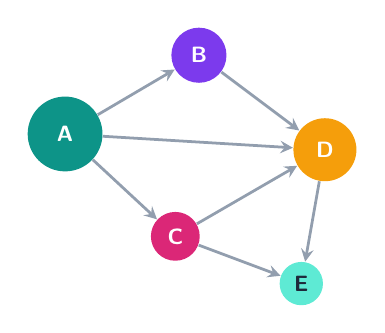
\begin{tikzpicture}[every node/.style={circle,draw=none,text=white,font=\bfseries\footnotesize,inner sep=0pt}]
      \node[fill=cTeal,minimum size=0.95cm]   (A) at (0,0)      {A};
      \node[fill=cPurple,minimum size=0.7cm]   (B) at (1.7,1.0)  {B};
      \node[fill=cPink,minimum size=0.62cm]    (C) at (1.4,-1.3) {C};
      \node[fill=cAmber,minimum size=0.8cm]    (D) at (3.3,-0.2) {D};
      \node[fill=cTealL,minimum size=0.55cm,text=cInk] (E) at (3.0,-1.9) {E};
      \foreach \a/\b in {A/B,A/C,A/D,B/D,C/D,D/E,C/E}
        \draw[->,>=stealth,cSlate!70,line width=1pt] (\a)--(\b);
    \end{tikzpicture}\\[3pt]
    {\tiny\color{cSlate}\itshape each page $=$ a state}
  \end{column}
  \begin{column}{0.54\textwidth}
    \begin{cblock}{cTeal}{The random surfer}\scriptsize
      Click links at random forever. \textbf{The fraction of time spent on each page} is its PageRank --- the page's importance.\\[4pt]
      \centering\color{cInk}$\text{PageRank}(p)=\pi(p),\quad \pi=\pi P$
    \end{cblock}
    \vspace{-0.3em}
    \begin{cblock}{cAmber}{The ``random teleport''}\scriptsize Google's damping factor is just a fix to guarantee \textbf{ergodicity} --- the exact condition from the previous slide.\end{cblock}
  \end{column}
\end{columns}
\end{frame}

% ----------------------------------------------------- MCMC
\begin{frame}[t]{MCMC: running the walk on purpose}
\kick{Killer app \#2}
\begin{columns}[t,onlytextwidth]
  \begin{column}{0.48\textwidth}
    \begin{dblock}{cTeal}{Forward (your assignment)}\centering\color{white} Given $P\ \rightarrow$ find $\pi$\par
      \scriptsize\color{cTealL}\itshape ``here are the rules; where do I end up?''\end{dblock}
  \end{column}
  \begin{column}{0.48\textwidth}
    \begin{dblock}{cPurple}{Inverse (MCMC)}\centering\color{white} Given $\pi\ \rightarrow$ design $P$\par
      \scriptsize\color{cTealL}\itshape ``I want this distribution; build a walk that lands there.''\end{dblock}
  \end{column}
\end{columns}
\vspace{0.3em}
\begin{cblock}{cPurple}{Why your ML team uses this every week}\scriptsize
\begin{columns}[t,onlytextwidth]
  \begin{column}{0.32\textwidth}\textbf{Bayesian posteriors.} Can't compute it? Sample it. Metropolis--Hastings \& Gibbs build a chain whose $\pi$ is the posterior.\end{column}
  \begin{column}{0.32\textwidth}\textbf{Diffusion models.} Image generators denoise via a learned Markov chain --- the same convergence guarantee, on pixels.\end{column}
  \begin{column}{0.32\textwidth}\textbf{LLM decoding.} Token-by-token sampling is a Markov process over text; temperature tunes the transition probabilities.\end{column}
\end{columns}
\end{cblock}
\end{frame}

% ----------------------------------------------------- hitting time
\begin{frame}[t]{Expected hitting time $=$ a linear system}
\kick{Station 4 \ \textbullet\ \ one more gem}
\small Q4(b): how long until the price first reaches $b$ from $a$? The recurrence $E_x=p_xE_{x+1}+r_xE_x+q_xE_{x-1}+1$ becomes a matrix equation.
\vspace{0.3em}
\begin{columns}[t,onlytextwidth]
  \begin{column}{0.46\textwidth}
    \begin{dblock}{cTeal}{Probability $\to$ Linear Algebra}\centering\color{white}\Large $A\,\mathbf{E}=\mathbf{1}$\par
      \scriptsize\color{cTealL}\itshape tridiagonal, except row $b$ pinned by $E_b=0$\par
      \vspace{3pt}\scriptsize\color{white} One solve answers infinitely many ``how long?'' questions --- the structure behind TD-learning targets.
    \end{dblock}
  \end{column}
  \begin{column}{0.5\textwidth}
    \begin{cblock}{cAmber}{``Hitting time'' shows up as\dots}\scriptsize
      \begin{itemize}\setlength\itemsep{2pt}
        \item[\textcolor{cAmber}{\textbullet}] \textbf{Churn} --- steps until a user reaches ``cancelled''
        \item[\textcolor{cAmber}{\textbullet}] \textbf{Reliability} --- mean time to failure
        \item[\textcolor{cAmber}{\textbullet}] \textbf{RL convergence} --- episodes to first reach the goal
        \item[\textcolor{cAmber}{\textbullet}] \textbf{Diffusion} --- time for info/infection to reach a node
      \end{itemize}
    \end{cblock}
  \end{column}
\end{columns}
\end{frame}

% ----------------------------------------------------- synthesis
\begin{frame}[t]{One idea, four disguises}
\kick{Zoom out}
\vspace{0.2em}
\begin{center}
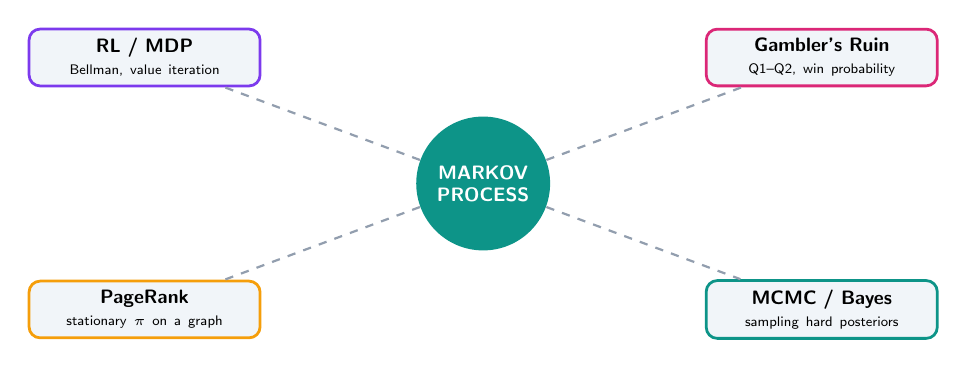
\begin{tikzpicture}
  \node[circle,fill=cTeal,text=white,font=\bfseries\scriptsize,align=center,minimum size=1.7cm] (M) at (0,0) {MARKOV\\PROCESS};
  \node[draw=cPurple,line width=1pt,rounded corners,fill=cLight,text width=2.7cm,align=center,font=\scriptsize] (RL) at (-4.3,1.6) {\textbf{RL / MDP}\\\tiny Bellman, value iteration};
  \node[draw=cPink,line width=1pt,rounded corners,fill=cLight,text width=2.7cm,align=center,font=\scriptsize] (GR) at (4.3,1.6) {\textbf{Gambler's Ruin}\\\tiny Q1--Q2, win probability};
  \node[draw=cAmber,line width=1pt,rounded corners,fill=cLight,text width=2.7cm,align=center,font=\scriptsize] (PR) at (-4.3,-1.6) {\textbf{PageRank}\\\tiny stationary $\pi$ on a graph};
  \node[draw=cTeal,line width=1pt,rounded corners,fill=cLight,text width=2.7cm,align=center,font=\scriptsize] (MC) at (4.3,-1.6) {\textbf{MCMC / Bayes}\\\tiny sampling hard posteriors};
  \foreach \n in {RL,GR,PR,MC} \draw[dashed,cSlate!70,line width=0.8pt] (M)--(\n);
\end{tikzpicture}
\end{center}
\centering\footnotesize\textit{\textcolor{cSlate}{Learn the atom once --- recognise it everywhere.}}
\end{frame}

% ----------------------------------------------------- discussion
\begin{frame}[t]{Questions to spark the room}
\kick{Let's discuss}
\small Conversation starters --- built on hooks your ML team already knows.
\vspace{0.5em}
\begin{columns}[t,onlytextwidth]
  \begin{column}{0.48\textwidth}\footnotesize
    \begin{itemize}\setlength\itemsep{8pt}
      \item[\textcolor{cTeal}{\textbullet}] If a fair coin gives win-prob $k/N$, why do casinos still always win?
      \item[\textcolor{cPurple}{\textbullet}] Where have you seen the Bellman ``max'' sneak into a model you've built?
      \item[\textcolor{cPink}{\textbullet}] What numerical-stability bug has bitten you --- a ``gambler's edge'' in disguise?
    \end{itemize}
  \end{column}
  \begin{column}{0.48\textwidth}\footnotesize
    \begin{itemize}\setlength\itemsep{8pt}
      \item[\textcolor{cAmber}{\textbullet}] Diffusion models are Markov chains in reverse --- does the stationary view reframe them?
      \item[\textcolor{cTeal}{\textbullet}] When is it worth running MCMC vs.\ just approximating the posterior?
      \item[\textcolor{cPurple}{\textbullet}] What ``expected hitting time'' would be most useful in our own systems?
    \end{itemize}
  \end{column}
\end{columns}
\end{frame}

% ----------------------------------------------------- takeaways
\begin{frame}[t]{What to walk away with}
\kick{Wrap-up}
\vspace{0.3em}
\begin{columns}[t,onlytextwidth]
  \begin{column}{0.48\textwidth}
    \begin{cblock}{cTeal}{01\ \ The Markov property is everywhere}\scriptsize ``Next depends only on now'' turns intractable problems into solvable recurrences.\end{cblock}
    \begin{cblock}{cAmber}{03\ \ Long-run behaviour $=\pi$}\scriptsize Stationary distributions rank web pages (PageRank) and let us sample anything (MCMC).\end{cblock}
  \end{column}
  \begin{column}{0.48\textwidth}
    \begin{cblock}{cPurple}{02\ \ Add a choice $\to$ you get RL}\scriptsize A gambler picking bets is an MDP. Value iteration is the same recurrence with a max.\end{cblock}
    \begin{cblock}{cPink}{04\ \ Representation is everything}\scriptsize Binary expansions, modular arithmetic, eigenvectors --- the right framing collapses complexity.\end{cblock}
  \end{column}
\end{columns}
\end{frame}

% ---------------------------------------------------------------- CLOSE
\begin{frame}[plain]
\begin{tikzpicture}[remember picture,overlay]
  \fill[cNavy] (current page.south west) rectangle (current page.north east);
  \fill[cTeal,opacity=0.15]   ([yshift=-2.4cm]current page.south west) circle (2.6cm);
  \fill[cPurple,opacity=0.15] ([yshift=2.0cm]current page.north east) circle (2.6cm);
  \node[anchor=west,text=cTealL,font=\scriptsize\bfseries] at ([shift={(0.95cm,2.2cm)}]current page.west) {THANK YOU};
  \node[anchor=west,text=white,font=\fontsize{26}{30}\selectfont\bfseries,text width=11cm]
     at ([shift={(0.9cm,1.05cm)}]current page.west) {From a coin flip to the frontier of ML};
  \node[anchor=west,text=cLight,font=\itshape\small,text width=10.5cm]
     at ([shift={(0.95cm,-0.35cm)}]current page.west)
     {The same four-line recurrence you solved in MTL106 is quietly running inside the models we build every day.};
  \node[anchor=north west,text=cTealL,font=\scriptsize\bfseries] at ([shift={(0.95cm,-1.3cm)}]current page.west) {GO DEEPER};
  \node[anchor=north west,text=cLight,font=\scriptsize,text width=11.5cm,align=left]
     at ([shift={(0.95cm,-1.7cm)}]current page.west)
     {\textbf{Sutton \& Barto} --- \emph{Reinforcement Learning} (Ch.~4, the Gambler's Problem)\\
      \textbf{arXiv:2001.00102} --- ``The Gambler's Problem and Beyond'' (its fractal value function)\\
      \textbf{Grinstead \& Snell} --- \emph{Introduction to Probability} (Ch.~12, Random Walks)};
  \node[anchor=south west,text=cTealL,font=\bfseries\small] at ([shift={(0.95cm,0.55cm)}]current page.south west) {Questions? Let's talk random walks.};
\end{tikzpicture}
\end{frame}

\end{document}